% !TEX program = lualatex
\documentclass{memoria}
\addbibresource{bib/references.bib}

\begin{document}
\memoriatitlepage{Memoria}{תוכנית עסקית והצעת מחיר\\ \en{AI Photo Restoration \& Family Archive Studio}}{נובמבר 2026}

\tableofcontents
\clearpage

\section{01-executive-summary}
Skeleton text. \en{English} \num{123}.
\nocite{placeholder}

\section{הבעיה והזדמנות השוק \en{(Problem \& Market)}}

\subsection{הבעיה}
תצלומים מודפסים מתכלים: הצבעים דוהים, הנייר נסדק, כתמי לחות ושריטות פוגעים בפרטי הפנים. בו־זמנית, רוב המשפחות אינן יודעות מי מופיע בתצלומים הישנים. כאשר הדור המבוגר נפטר, השמות, המקומות והסיפורים נעלמים יחד איתו. הפתרונות הקיימים מתחלקים לשלושה סוגים, וכל אחד מהם חלקי.

\begin{table}[h]
\centering
\caption{השוואה בין חלופות קיימות לבין \en{Memoria}}
\label{tab:alternatives}
\small
\begin{tabularx}{\textwidth}{>{\bfseries}l X X X}
\toprule
\theadrow \thead{חלופה} & \thead{יתרון} & \thead{חסרון} & \thead{פער ש-\en{Memoria} סוגרת} \\
\midrule
סריקה עצמית בבית & זולה & איכות נמוכה, ללא שחזור & סריקה ארכיונית ושחזור \\
\en{Photoshop} ידני & תוצאה איכותית & יקר וארוך, כ-\num{2} שעות לתמונה & אוטומציה בסיוע \en{AI}, עם בקרת אדם \\
אפליקציות \en{AI} כלליות & מהירות & אין ארכיון, אין שירות, פרטיות לא ברורה & ארכיון מתועד והסכמה מפורשת \\
\bottomrule
\end{tabularx}
\end{table}

\subsection{פלח הלקוחות}
אנו מתמקדים בשלושה פלחים. הראשון הוא \emph{משפחות מורחבות} המתכננות אירוע (יום הולדת של סבתא, יום נישואין, שבעה) ורוצות אלבום ייחודי. השני הוא \emph{בני דור ביניים} בגילאי \num{40--60} המנקים בית של הורים. השלישי הוא \emph{ארגונים קטנים}: קיבוצים, מושבים, בתי כנסת ואגודות קהילתיות המחזיקים ארכיונים היסטוריים.

\subsection{אומדן שוק}
הערה מתודולוגית: אין בידינו נתון פומבי אמין על היקף שוק השחזור בישראל, ולכן אנו מציגים אומדן הנדסי ולא ציטוט. נניח \num{3.5} מיליון משקי בית בישראל, ושיעור קטן מהם, \num{0.5}\%, פונה לשירות מסוג זה בשנה. התוצאה היא כ-\num{17{,}500} לקוחות פוטנציאליים בשנה. מחיר הזמנה ממוצע של \num{\MAvgOrderPrice} ש״ח מציב את הפוטנציאל השנתי בסדר גודל של \num{13.7} מיליון ש״ח. שיעור החדירה שאנו מתכננים הוא כ-\num{\MOrdersEnd} הזמנות בחודש בסוף השנה השלישית, כלומר פחות מ-\num{15}\% מהפוטנציאל המשוער. נציין שהנחה זו נבדקת בניתוח הרגישות בפרק הפיננסי.

\subsection{יתרון תחרותי}
\begin{enumerate}[leftmargin=*]
  \item \textbf{שירות מלא} ולא כלי: סריקה, שחזור, תיעוד וגיבוי במקום אחד.
  \item \textbf{בקרת אדם} על כל תמונה לפני מסירה, כדי למנוע ״הזיות״ של מודל השחזור בפני אדם אמיתי.
  \item \textbf{פרטיות כברירת מחדל}: עיבוד מקומי, מחיקה לפי בקשה, והסכמה כתובה.
  \item \textbf{תמחור שקוף} ברמת הזמנה, ללא הפתעות.
\end{enumerate}

\subsection{דמויות לקוח}
\begin{figure}[h]
\centering
\begin{tikzpicture}[
  card/.style={draw=mteal,fill=mpaper,rounded corners=4pt,text width=0.30\textwidth,inner sep=7pt,font=\small,line width=0.8pt,align=center}]
  \node[card] (p1) {\textbf{\sffamily רונית, \num{58}}\\ סבתא לשמונה נכדים\\[2pt] רוצה אלבום ליום ההולדת של בעלה. מוכנה לשלם עבור איכות ושקט נפשי.};
  \node[card,right=4mm of p1] (p2) {\textbf{\sffamily דן, \num{47}}\\ מנקה את בית ההורים\\[2pt] מצא שלוש קופסאות תמונות ואינו יודע מי מופיע בהן. מחפש פתרון מקיף.};
  \node[card,right=4mm of p2] (p3) {\textbf{\sffamily ועד הקיבוץ}\\ ארכיון היסטורי\\[2pt] מעוניין בסריקה של \num{800} תמונות ובמטא־נתונים לשימוש ציבורי.};
  \foreach \p in {p1,p2,p3} \fill[mamber] ([yshift=-1.5pt]\p.north west) rectangle ([yshift=0pt]\p.north east);
\end{tikzpicture}
\caption{שלוש דמויות לקוח מייצגות, מבוססות על הפלחים שהוגדרו. הדמויות בדויות ונועדו לתכנון שירות.}
\label{fig:personas}
\end{figure}

כל דמות מובילה לחבילה אחרת: רונית ל-\en{Heritage} עם אלבום מודפס, דן ל-\en{Pro} בהיקף של כמה הזמנות, והקיבוץ להסכם ארגוני עם הנחת כמות. הדמויות משמשות אותנו גם כמבחן קבלה לתהליך: לכל אחת נכתב תסריט שימוש מקצה לקצה, וכל שלב בו נבדק מול ציפיות הלקוחה או הלקוח.

\section{השירות ותהליך העבודה \en{(Service \& AI Pipeline)}}

\subsection{סקירת התהליך}
התהליך מורכב משישה שלבים. כל שלב מייצר תוצר ביניים הנשמר בארכיון, כך שאפשר לחזור אחורה ולהשוות מקור מול תוצאה.

\begin{figure}[h]
\centering
\begin{english}\begin{tikzpicture}[
  node distance=4mm,
  pstep/.style={draw=mteal,fill=mpaper,rounded corners=3pt,minimum width=21mm,minimum height=12mm,align=center,font=\sffamily\scriptsize,line width=0.8pt},
  hum/.style={pstep,fill=mamber!25,draw=mamber},
  arr/.style={-{Stealth[length=2mm]},line width=0.9pt,color=mtealdark}]
  \node[pstep] (a) {Intake\\ and consent};
  \node[pstep,right=of a] (b) {Scan\\ 1200 dpi};
  \node[pstep,right=of b] (c) {AI\\ restore};
  \node[hum,right=of c] (d) {Human\\ review};
  \node[pstep,right=of d] (e) {Archive\\ and metadata};
  \node[pstep,right=of e] (f) {Delivery};
  \foreach \x/\y in {a/b,b/c,c/d,d/e,e/f} \draw[arr] (\x) -- (\y);
  \draw[arr,dashed,color=msepia] (d.south) -- ++(0,-8mm) -| node[pos=0.25,below,font=\sffamily\tiny]{rework loop} (c.south);
\end{tikzpicture}\end{english}
\caption{תהליך העבודה של \en{Memoria}. השלב הצהוב הוא בקרת אדם; החץ המקווקו מציין חזרה לשחזור מחדש.}
\label{fig:pipeline}
\end{figure}

\subsection{פירוט השלבים}
\paragraph{קליטה והסכמה.} כל הזמנה נפתחת בטופס הסכמה: מי בעל הזכויות בתמונות, האם מותר לעבד תמונות של אנשים מזוהים, ומה מדיניות המחיקה. הלקוח מקבל מספר הזמנה ומדבקת מעקב.

\paragraph{סריקה.} הסריקה מתבצעת ברזולוציה של \num{1200}~\en{dpi} לפחות לתצלומים קטנים, בפורמט \en{TIFF} ללא דחיסה. קובץ המקור נשמר ולעולם אינו נדרס, בהתאם לעיקרון ״המקור הוא קדוש״.

\paragraph{שחזור בסיוע \en{AI}.} השלב משלב שלושה מודלים: הגדלת רזולוציה והסרת רעש \cite{wang2021realesrgan}, שחזור פנים \cite{wang2021gfpgan}, וצביעה אופציונלית \cite{zhang2016colorful}. הצבעים שמוצעים בצביעה הם \emph{פרשנות} ולא עובדה; לכן הם מסומנים כך בארכיון.

\paragraph{בקרת אדם.} מומחה בודק כל תמונה בהגדלה, משווה פנים למקור, ומאשר או מחזיר לעיבוד. זהו שלב הבקרה המרכזי, והוא מאפיין את ההצעה שלנו מול כלי \en{AI} אוטומטיים.

\paragraph{ארכיון ומטא־נתונים.} כל תמונה מתויגת: שמות, מקום, תאריך משוער, מקור, והערות המשפחה. התיעוד נשמר בפורמט פתוח (\en{JSON} ו-\en{CSV}) כדי שלא יהיה קשר ל-\en{Memoria} אם הלקוח יעבור ספק.

\paragraph{מסירה.} הלקוח מקבל קישור מוצפן להורדה, כונן \en{USB} ואלבום מודפס בחבילת \en{Heritage}. הגיבוי נשמר בענן לתקופה שנקבעה בחוזה.

\subsection{מדדי איכות}
\begin{table}[h]
\centering
\caption{מדדי שירות מתוכננים}
\label{tab:sla}
\small
\begin{tabularx}{0.9\textwidth}{>{\bfseries}X l l}
\toprule
\theadrow \thead{מדד} & \thead{יעד} & \thead{שיטת מדידה} \\
\midrule
זמן אספקה, חבילת \en{Basic} & עד \num{5} ימי עבודה & חותמת זמן בקליטה ובמסירה \\
זמן אספקה, חבילת \en{Heritage} & עד \num{15} ימי עבודה & חותמת זמן בקליטה ובמסירה \\
תמונות שהוחזרו לשחזור מחדש & מתחת ל-\num{8}\% & יומן בקרת אדם \\
שביעות רצון לקוח & \num{4.6} מתוך \num{5} ומעלה & סקר לאחר מסירה \\
\bottomrule
\end{tabularx}
\end{table}

\subsection{איך מודדים איכות שחזור}
״נראה טוב״ אינו מדד מספיק לעסק. לכן אנו מגדירים מדדים כמותיים. המדד הנפוץ הוא יחס אות לרעש שיא (\en{PSNR}):
\begin{equation}
  \mathrm{PSNR} \;=\; 10\log_{10}\!\left(\frac{\mathrm{MAX}^2}{\mathrm{MSE}}\right), \qquad
  \mathrm{MSE} = \frac{1}{HW}\sum_{i,j}\bigl(x_{ij}-\hat{x}_{ij}\bigr)^2 ,
\end{equation}
כאשר $x$ התמונה המקורית ו-$\hat{x}$ התמונה המשוחזרת. מדד משלים הוא דמיון מבני (\en{SSIM}), המשווה בהירות, ניגודיות ומבנה:
\begin{equation}
  \mathrm{SSIM}(x,y) \;=\; \frac{(2\mu_x\mu_y + c_1)(2\sigma_{xy} + c_2)}{(\mu_x^2+\mu_y^2 + c_1)(\sigma_x^2+\sigma_y^2 + c_2)} .
\end{equation}
מדדים אלה דורשים תמונת ייחוס נקייה, שאין לנו בתצלומים אמיתיים. לכן ביצענו ניסוי סינתטי: יצרנו בקוד ״תצלום״ מלאכותי, הוספנו רעש וקווי שריטה, והפעלנו מסנן קלאסי פשוט (חציון אופקי וטשטוש ממוצע). זהו קו בסיס ולא המודל שלנו; הוא נועד להדגים כיצד נמדד שיפור. ה-\en{PSNR} עלה מ-\num{\QPsnrBefore}\,\en{dB} ל-\num{\QPsnrAfter}\,\en{dB}, וה-\en{SSIM} הגלובלי מ-\num{\QSsimBefore} ל-\num{\QSsimAfter}.

\begin{figure}[h]
\centering
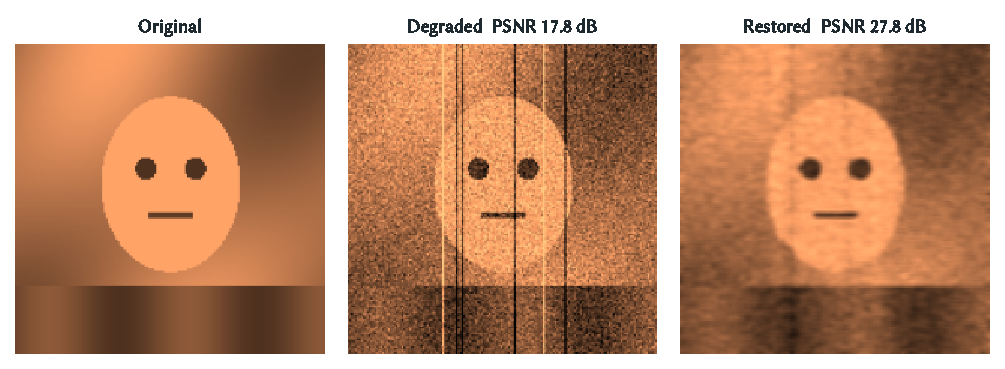
\includegraphics[width=\textwidth]{figures/quality_demo.pdf}
\caption{ניסוי סינתטי: מקור, גרסה פגועה ותוצאת מסנן קלאסי. כל התמונות נוצרו בקוד (\code{code/quality\_demo.py}) ללא תמונות חיצוניות.}
\label{fig:qdemo}
\end{figure}

\begin{figure}[h]
\centering
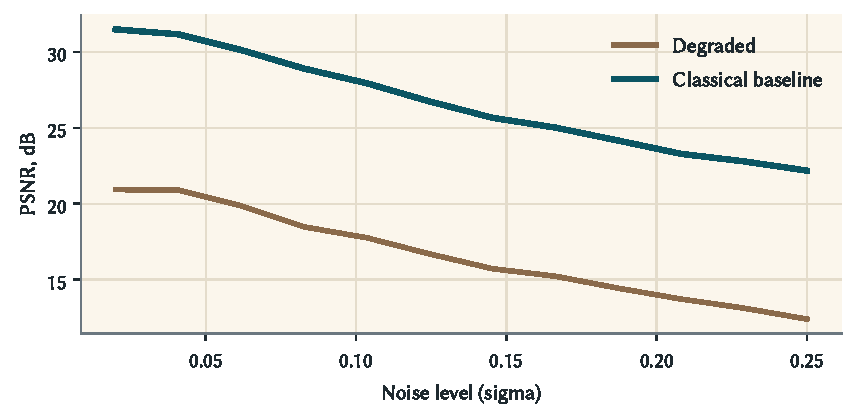
\includegraphics[width=0.72\textwidth]{figures/quality_curve.pdf}
\caption{שיפור \en{PSNR} של קו הבסיס הקלאסי כפונקציה של עוצמת הרעש. ככל שהרעש חזק יותר, השיפור המוחלט קטן, ולכן שחזור קשה דורש מודלים מתקדמים ובקרת אדם.}
\label{fig:qcurve}
\end{figure}

בפועל נשתמש במדדים אלה לבדיקות רגרסיה: אוסף קטן של תמונות בדיקה מדודות מורץ מחדש בכל שדרוג מודל, ושדרוג המוריד את המדדים נדחה. על גבי המדדים הכמותיים מוסיפה בקרת האדם את מה שמספרים אינם רואים: האם הפנים עדיין דומים לאדם האמיתי.

\section{04-pricing}
Skeleton text. \en{English} \num{123}.
\nocite{placeholder}

\section{05-financials}
Skeleton text. \en{English} \num{123}.
\nocite{placeholder}

\section{06-gtm-operations}
Skeleton text. \en{English} \num{123}.
\nocite{placeholder}

\section{07-risks-privacy}
Skeleton text. \en{English} \num{123}.
\nocite{placeholder}

\section{08-conclusion}
Skeleton text. \en{English} \num{123}.
\nocite{placeholder}

\section{A-quote}
Skeleton text. \en{English} \num{123}.
\nocite{placeholder}


\printbibliography[title={ביבליוגרפיה}]
\end{document}
